% @author Arian Helberg

\chapter{Konzepte}
Mit der Erstellung eines Programms zur Synthetisierung von Ähnlichkeitsabbildungen einer vom Benutzer
erstellten Verzweigungsstruktur soll die Praktikabilität aktueller Forschungsansätze untersucht werden.
\\~\\
Folgende Kernkonzepte werden erläutert und umgesetzt:
\begin{itemize}
    \item Visualisierung und prozessorientiertes Erstellen von Basisstrukturen,
    \item Organisation in einer prozessoptimierten, baumähnlichen Topologie,
    \item L-System-Repräsentationen,
    \item Algorithmen zur Inferierung, Komprimierung, Generalisierung und
    \item Verarbeitung von Transformationsparametern
\end{itemize}

\section{Probleme \& Lösungsansätze}
\label{probleme}

\subsection*{Visualisierung}
Um eine geführte Erstellung der Basisstruktur zu ermöglichen, muss diese während der Erstellung sichtbar gemacht werden.
Hierzu werden die Templates in Form von Zeichenketten angelegt und mittels Turtle-Grafik visualisiert.
Eine Turtle-Grafik beschreibt die Interpretation einer Zeichenkette als Bild durch Ausführen eines Logo-Turtle-Algorithmus.
Weiter wird auch zur Evaluation der Ergebnisse eine Visualisierung benötigt.
Da die Verzweigungsstrukturen in L-System-Repräsentation vorliegen, wird hierzu eine Interpretationsfunktion benötigt,
die diese Ersetzungssysteme in Bildform darstellen.
Ein L-System wird durch Ausführung in eine erweiterte Zeichenkette überführt und als Turtle-Grafik beschrieben
~\cite{prusinkiewicz_1986}.

\subsection*{Basisstruktur}
Der Benutzer verwendet grafische Bendienelemente, um eingelesene Templates auszuwählen, Transformationsparameter anzupassen
und anschließend die Instanzen der Basisstruktur hinzuzufügen.
Im Folgenden wird diese Basisstruktur u.a. Grundstruktur oder Eingabestruktur genannt.

\subsection*{Baumstruktur}
Um Grundstrukturen mittels verschiedener Algorithmen untersuchen zu können, werden die einzelnen Template-Instanzen in
einer baumähnlichen Struktur organisiert.
Transformationsparameter einer Instanz beschreiben die räumlichen Veränderungen gegenüber des zugrundeliegenden Templates
und haben daher keine Aussagekraft in Bezug auf die Strukturtopologie der Basisstruktur.
Der Fokus dieser Arbeit liegt auf topologischen\\Eigenschaften von Verzweigungsstrukturen (z.B. Rekursion).
Darum bilden die einzelnen Template-Instanzen die Knoten der Baumtopologie, während die Kanten die räumlichen Transformationen
darstellen.
So wird eine datenstrukturelle Trennung zwischen Topologie und räumlicher Transformationen geschaffen.
Diese baumähnliche Struktur ist inspiriert durch die Arbeit von~\citeauthor{guo_2020}~\cite{guo_2020}.

\subsection*{Inferieren}
Das Smallest Grammar Problem, also das Finden der kleinsten, kontextfreien Grammatik, welche eine bestimmte Zeichenkette
generiert, ist ein offenes Problem der Informatik~\cite{charikar_2005}.
Primär wird in der Forschung nach Algorithmen gesucht, die ein akzeptables Ergebnis liefern.
In dieser Arbeit wird ein Algorithmus präsentiert, der die Knoten der Baumstruktur in einzelne Symbole umwandelt, mit
Produktionsregeln verknüpft und diese dem resultierenden L-System hinzufügt.
Dieses L-System repräsentiert lediglich die Eingabestruktur.

\newpage

\subsection*{Komprimieren}
Zur Erzeugung eines kompakten, gewichteten L-Systems werden sich wiederholende\\Unterbäume gesucht und ersetzt.
Um das zu erzeugende L-System mit einer kleinen oder großen Regelmenge auszustatten, wird eine Gewichtung angewendet.
Eine Kostenfunk-tion stellt hierbei die Anzahl Symbole aller RHS der Produktionsregeln mit der Menge an Anwendungen der
LHS gegenüber.

\subsection*{Generalisieren}
Da das kompakte L-System eine Repräsentation der vom Benutzer erzeugten Verzweigungsstruktur darstellt, werden ähnliche
Regeln miteinander verbunden (Merge) und mit einer Wahrscheinlichkeit versehen, um nicht-deterministische Regeln hinzuzufügen.
Eine weitere Kostenfunktion bewertet den Merge zweier Produktionregeln.
Sie wendet eine Gewichtung über die Länge der Grammatik zur Änderungsdistanz von der alten (ohne Merge) zur neuen Grammatik an.

\subsection*{Transformationen}
Die vom Benutzer vergebenen Werte der Transformationsparameter werden während der Erstellung der Eingabestruktur in
einer Häufigkeitsverteilung organisiert und bei Ausführung des generalisierten L-Systems angewendet.
So werden Transformationen nach ihrer statistischen Häufigkeit eingesetzt.

\newpage

\section{Workflows \& Algorithmen}
\label{algo}

\subsubsection*{Verzweigungsstruktur erstellen}
Um als Benutzer des Systems eine Verzweigungsstruktur zu erstellen, wird folgender Arbeitsablauf umgesetzt:
\begin{algorithm}[caption={Erstellen einer Verzweigungsstruktur}, label={alg1}]
    Erster Anker ist vorselektiert
    Wiederhole, bis Struktur fertiggestellt ist:
        Selektiere ein Template aus der Liste
        Setzte Parameter
        Bestätige Auswahl und Parameter
        Zeichne ausgewähltes Template mit Parametern
        Wähle nächsten Anker aus
\end{algorithm}

\subsubsection*{L-System inferieren}
Aus der Verzweigungsstruktur kann nun ein L-System erzeugt werden.
Hierzu wird ein neuer Algorithmus (siehe Algorithmus 32) präsentiert:\\~\\
Zunächst werden L-System-Komponenten erzeugt (Zeile 2-6) für $\mathcal{L}=\langle M,\omega,R \rangle$:
\begin{itemize}
    \item Das Alphabet wird mit den Symbolen F und S initialisiert, da F als Repräsentation einer grundlegenden
    Zeichenoperation und S als Axiom in jeder Anwendung des Algorithmus vorkommt.
    \item Die erste Produktionsregel $\alpha$ umfasst die Abbildung des Axioms auf ein neues Symbol, das nicht im Alphabet
    vorkommt.
    Das Alphabet wird stets um ein Symbol lexikografischer Ordnung ergänzt:
    \begin{itemize}
        \item Bsp.: $\{A,B,C\}$ wird ein neues, unbekanntes Symbol hinzugefügt $\rightarrow \{A,B,C,D\}$
    \end{itemize}
    \item Die Variable $\beta$ hält zu untersuchende Knoten der Baumtopologie, welche nach Breitensuche iteriert werden.
    Der erste Durchlauf startet bei Wurzelknoten S.
    \item Als letzter Schritt der Initialisierung wird dem Alphabet ein neues Symbol hinzugefügt, das durch die Variable
    $\gamma$ gehalten wird.
\end{itemize}
Die Schleife des Algorithmus beschäftigt sich mit der Iterierung des Baumes und dem Erstellen neuer Symbole und
Produktionsregeln für das resultierende L-System (Zeile 8-17):
\begin{itemize}
    \item Die in den Knoten des Baumes gehaltenen Template-Instanzen entprechen einer Zeichenkette, die durch eine
    Turtle-Grafik interpretiert, einem vom Benutzer transformierten Template entspricht.
    Diese Zeichenkette wird in $\delta$ gespeichert.
    \item In Zeile 9-12 wird die genannte Zeichenkette auf Verzweiungsvariablen ($A-Z$; $F$ ausgeschlossen) untersucht.
    Ein neues Symbol ersetzt das dem Alphabet hinzugefügte Symbol. Anschließend wird eine Produktionregel,
    die auf die veränderte Zeichenkette abbildet, der Produktionsregelmenge hinzugefügt.
    \item Zeile 13 prüft, ob es ein Symbol im Alphabet gibt, das nicht als Ziel einer Produk-tionsregel in der Produktionsregelmenge
    definiert ist. In diesem Fall wird das Symbol als Ziel der nächsten Produktion gesetzt. Andernfalls schließt der Algorithmus ab.
    \item Das Schleifen-Attribut ist das Setzen des nächsten Knotens am Ende der Schleife (Zeile 17).
\end{itemize}

\begin{algorithm}[caption={Inferieren eines L-Systems aus einer Baumstruktur}, label={alg2}]
    Initialisierung:
        $M=\{F,S\}$
        $\omega=S$
        $R \gets \{\alpha$: $S \rightarrow A\}$
        $\beta=$ nächster Knoten
        $M \gets \gamma \in \{A,B,\dots,Z\}$, mit $\gamma \notin M$
    Schleife:
        $\delta=$ Wort von $\beta$
        $\forall \{A,B,\dots,Z\} \setminus F \in \delta:$
        Ersetze mit $\zeta \in \{A,B,\dots,Z\}$, mit $\zeta \notin M$
        $M \gets \zeta$
        $R \gets \{\gamma\rightarrow\delta\}$
        Wenn es ein Symbol $\eta$ in $M\setminus\{F,S\}$ gibt mit $\{\eta \rightarrow bel.\} \notin R$:
            $\gamma=\eta$
        Sonst:
            Breche Schleife ab
        $\beta=$ nächster Knoten
\end{algorithm}

\subsubsection*{L-System komprimieren}
\citeauthor{guo_2020} führt einen Algorithmus zum Inferieren einer Grammatik aus einer Baumstruktur ein~\cite{guo_2020}.
Zum Einen wird ein L-System aufgebaut, zum Andern die Baumtopologie durch Finden maximaler Subbäume reduziert.
Diese Reduktion wird im folgenden Algorithmus (siehe Algorithmus 33) adaptiert:\\~\\
Initialisierung (Zeile 2-5):
\begin{itemize}
    \item Das L-System, welches der Eingabe des Algorithmus entspricht, wird ausgeführt und
    die resultierende Zeichenkette wird in $\mathcal{L^+}$ gespeichert.
    \item Ein Parameter $w_l$ wird eingeführt, der eine Kostenfunktion (Zeile 11) nach Anzahl an Symbolen
    der RHS von Produktionsregeln und die Anzahl deren Anwendung gewichten soll.
    \item Anschließend wird ein maximaler Subbaum durch geschachtelte Iteration des Baumes $T$ gesucht und als $T'$ gesetzt.
    \item Es werden ausschließlich maximale Unterbäume behandelt, die mindestens zweimal im Baum vorkommen.
\end{itemize}
Die Schleife (Zeile 7-13) stellt die Reduzierung dar:
\begin{itemize}
    \item Zunächst werden alle Vorkommen des maximalen Unterbaumes durch ein neues Symbol ersetzt.
    \item Aus diesem Subbaum wird ein L-System inferiert, das wiederum in eine erweiterte Zeichenkette ausgeführt wird.
    \item Die Zeichenkette wird als LHS einer neuen Produktionsregel gesetzt, die auf das neue Symbel abzielt.
    \item Das alte L-System kann nun mit dem veränderten L-System mittels Kostenfunktion verglichen werden (Zeile 9):
    Liegen die Kosten des veränderten L-Systems unter den Kosten des Alten, wird die Reduktion beendet.
    Andernfalls gilt der Subbaum nun als Eingabebaum und das veränderte Ersetzungssystem als Eingabe-L-System.
\end{itemize}

\begin{algorithm}[caption={Erstellen eines kompakten L-Systems mit Gewichtung $w_l$}, label={alg3}]
Initialisierung:
    $\mathcal{L}^+ \leftarrow L_s$
    $\mathcal{L}=\emptyset$
    Setze Gewichtungsparameter $w_l \in [0,1]$
    Finde maximalen Unterbaum $T'$ aus $T$ mit Wiederholungen $n>1$
Schleife (Reduzierung):
    Ersetze alle Vorkommen von $T'$ mit demselben Symbol $\gamma \in \{A,B,\dots,Z\}$
    $R \leftarrow \{\gamma \rightarrow L_s\}$ mit $L_s$ aus $T'$, $R$ aus $\mathcal{L}$
    Wenn $C_i(\mathcal{L}) \geq C_i(\mathcal{L}^+)$:
        Breche Schleife ab
    $T \leftarrow T'$
    $\mathcal{L}^+ \leftarrow \mathcal{L}$
    Finde maximalen Unterbaum $T'$ aus $T$ mit Wiederholungen $n>1$
\end{algorithm}

\begin{algorithm}[caption={Kostenfunktion $C_i$ mit Gewichtung $w_l$}, label={alg4}]
$C_i(\mathcal{L})= \sum\limits_{A(P) \rightarrow M^* \in \mathcal{L}} w_l * |M^*| + (1 - w_l) * N(A(P)\rightarrow M^*)$
\end{algorithm}
$N(\cdot)$ dient als Zählfunktion für die Anzahl Wiederholungen einer \textit{LHS} in einem ausgeführten L-System.

\subsubsection*{L-System generalisieren}
Da das kompakte L-System eine Repräsentation der vom Benutzer erzeugten Verzweigungsstruktur darstellt, werden
nun ähnliche Regeln miteinander verbunden und mit\\einer Wahrscheinlichkeit versehen, um nicht-deterministische
Regeln hinzuzufügen.\\
Sowohl Längenfunktionen, Kostenfunktionen und Distanzalgorithmen, als auch der Grund-algorithmus sind aus einer Arbeit
von~\citeauthor{guo_2020} entnommen und bauen sich wie folgt auf~\cite{guo_2020}:

\begin{itemize}
    \item Die Längenfunktion $L$, die auf eine Grammatik angewendet wird, summiert die Anzahl Symbole des Alphabets mit
    der Anzahl an RHS der Produktionsregeln. Sie berechnet somit die Gesamtheit aller Symbole, die das L-System abbilden soll.
    (Länge der Grammatik).
    \item Der Abstand zweier Zeichenketten kann mit der \textit{String Edit Distance} ermittelt werden. Diese wird über
    die Funktion $D_s$ abgebildet. Hierbei wird die Anzahl an Operationen summiert, die für die Überführung einer Zeichenkette
    in eine Andere nötig sind (Zeichenkettenaustausch, -einschub und -löschung)
    \item Mit $D_s$ kann nun auch der Abstand zweier Grammatiken zueinander bestimmt werden. Diese Funktion wird mit
    $D_g$ abgebildet.
    \item Die Kostenfunktion $C_g$ nutzt die Länge und Distanz von Grammatiken, um Kosten einer Überführung von einer Grammatik
    in eine andere messen zu können. Sie berechnet somit die Kosten, um $L^*$ in $L^+$ zu überführen.
    Der Parameter $w_0$ gewichtet hierbei die Differenz der Länge der Grammatiken und die Anzahl Operationen, die zur
    Überführung nötig sind. Die Überführungskosten werden in der Variable $C^{old}_g$ zur Verfügung gestellt.
\end{itemize}

\begin{algorithm}[caption={Längenfunktion $L$ für Grammatiken}]
$L(\mathcal{L}) = |M| + \sum\limits_{A(P) \rightarrow M^* \in \mathcal{L}} |M^*|$
\end{algorithm}

\begin{algorithm}[caption={Grammar Edit Distance}]
$D_g(\mathcal{L}^+, \mathcal{L}^*)= \sum\limits_{(A(P) \rightarrow M^*_A , B(P) \rightarrow M^*_B) \in M(\mathcal{L^+} \rightarrow \mathcal{L^*})} D_s(M^*_A, M^*_B)$
\end{algorithm}

\begin{algorithm}[caption={Kostenfunktion $C_g$ mit Gewichtung $w_0$}]
$C_g(\mathcal{L}^*, \mathcal{L}^+) = w_0 * (L(\mathcal{L}^*) - L(\mathcal{L}^+)) + (1 - w_0) + D_g(\mathcal{L}^+, \mathcal{L}^*)$
\end{algorithm}

\newpage

Algorithmus 38 zum Generalisieren eines L-Systems:\\~\\
Initialisierung (Zeile 2-4):
\begin{itemize}
    \item Das zu untersuchende Tuple besteht aus zwei Produktionsregeln (Regelpaar) und wird in der Variable $p^*$ gehalten.
    \item L-Systeme, die sich infolge eines Merges geändert haben, werden in $L^+$ und Eingabe-L-Systeme in $L^*$ gespeichert.
\end{itemize}
Generalisierung (Zeile 6-13):
\begin{itemize}
    \item $\mathcal{P}$ ist die Menge aller möglichen Regelpaare aus $L^*$.
    \item Das Regelpaar, das beim Merge die geringsten Kosten für die Überführung in die neue Grammatik aufweist, wird in
    $p^*$ gehalten.
    \item Sind diese Kosten positiv, wird die Generalisierung abgebrochen.
    \item Andernfalls werden die Variablen $c^*$ als Delta-Kosten, $C^{old}_g$ und $L^*$ entsprechend gesetzt.
    \item Sollte die Differenz der Überführungskosten positiv sein, wird die Generalisierung abgebrochen.
\end{itemize}

\begin{algorithm}[caption={Generalisieren eines L-Systems mit Gewichtung $w_0$}]
Initialisierung:
    Regelpaar $p^* = \emptyset$
    $\mathcal{L}^* = \mathcal{L}^+$
    $C_g^{old} = C_g(\mathcal{L}^* + \{p^*\}, \mathcal{L}^*)$
Schleife:
    Finde Regelpaar $p^*$ mit minimalen Kosten $C_g(\mathcal{L}^* + \{p_i\}, \mathcal{L}^*), \forall p_i \in \mathcal{P}$
    Wenn $C_g(\mathcal{L}^* + \{p^*\}, \mathcal{L}^*) \geq 0$:
        Breche Schleife ab
    $c^* = C_g(\mathcal{L}^* + \{p^*\}, \mathcal{L}^*) - C_g^{old}$
    $C_g^{old} = C_g(\mathcal{L}^* + \{p^*\}, \mathcal{L}^*)$
    $\mathcal{L}^* = \mathcal{L}^* + \{p^*\}$
    Wenn $c^* > 0$:
        Breche Schleife ab
\end{algorithm}

\newpage

\section{Softwaretechnik}

\subsection*{Extreme Programming}
Eine Fallstudie der Universität Karlsruhe~\cite{muller_2001} untersucht den Einsatz der Softwaretechnik Extreme
Programming (XP) im Kontext der Erstellung von Abschlussarbeiten im Universitätsumfeld.
Hierzu werden folgende Schlüsselpraktiken untersucht:
\begin{itemize}
    \item XP als Softwaretechnik zur schrittweisen Annäherung an die Anforderungen eines Systems
    \item Änderung der Anforderungen an das System
    \item Funktionalitäten (Features) werden als Tätigkeiten des Benutzers (User Stories) definiert
    \item Zuerst werden Komponententests (Modultests) geschrieben und anschließend die Features (Test-driven Design)
    \item Keine seperaten Testing-Phasen
    \item Keine formalen Reviews oder Inspektionen
    \item Regelmäßige Integration von Änderungen
    \item Gemeinsame Implementierung (Pair Programming) in Zweiergruppen
\end{itemize}
Aus der Fallstudie geht hervor, dass Extreme Programming einige Vorteile bei der Bearbeitung eines Softwareprojektes
einer Bachelorarbeit bietet.
Zum Einen können sich Anforderungen an das zu erstellende System durch parallele Literaturrecherche ändern, zum
Anderen können Arbeitspakete durch Releases abgebildet werden.
Diese Softwaretechnik wird in der Umsetzung des Softwareprojekts zu dieser Arbeit angewendet.

\begin{figure}[H]
    \centering
    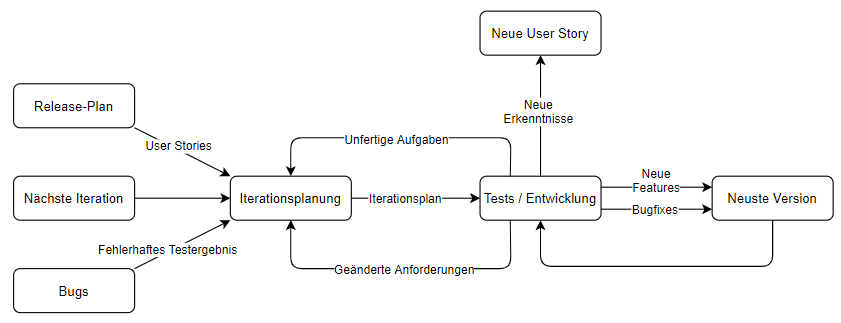
\includegraphics[width=12.8cm]{../images/extreme_programming.png}
    \caption{Zyklische Umsetzung des Softwareprojektes}
\end{figure}

\section{Softwarearchitektur}
Die Gliederung der Inhalte für die Softwarearchitektur erfolgt nach der arc42-Vorlage~\cite{arc42}.

\subsection*{Qualitätsziele}
Um die wesentlichen Features des Systems in einem Programm umzusetzen, werden Qualitätsziele in einem Qualitätsbaum
(siehe~\ref{baum}) definiert und Szenarien zugeordnet (Nummerierung).
Die nichtfunktionalen Anforderungen sind nach der DIN-Norm \texttt{DIN 66272} strukturiert.\\~\\
Der Benutzer ist in der Lage eine Verzweigungsstruktur zu erstellen, aus der dann eine oder mehrere ähnliche Strukturen
erzeugt werden können \textbf{(1)}.
Vordefinierte Templates sollen verwendet werden, um die Basisstruktur zu erzeugen \textbf{(2)}.
Dabei soll der Benutzer visuelles Feedback während des Erstellungsprozesses bekommen \textbf{(3)}.
Für den Benutzer besteht die Möglichkeit Parameter zu setzen, die die resultierenden Ähnlichkeitsstrukturen beeinflussen,
um so zu einem akzeptablen Ergebnis zu gelangen \textbf{(4)}.
Es soll nicht möglich sein eine ungültige Verzweigungsstruktur zu erstellen \textbf{(5)}.
Der Erstellungsvorgang soll jeder Zeit neu begonnen werden können, ohne das Programm neu starten zu müssen \textbf{(6)}.
Weiter sollte das Programm robust gegenüber Benutzereingaben sein \textbf{(7)}.
Eine intuitive Nutzung des Programms soll gegeben sein, sodass der Benutzer wenig Zeit für die Nutzung der Bedienelemente
aufbringen muss \textbf{(8)}.
Das Erzeugen der Struktur aus Kapitel~\ref{eval} (Evaluierung) soll ohne händische Nachbildung möglich sein \textbf{(9)}.\\
Zur Nachvollziehbarkeit sollten die verschiedenen L-System-Varianten in der Systemkonsole ausgegeben werden \textbf{(10)}.
Der Generierungsprozess nach dem Erstellen der Basis-struktur sollte nicht länger als vier Sekunden in Anspruch nehmen \textbf{(11)}.
Auch Fließkommazahlen sollte der Benutzer als Parameter festlegen können \textbf{(12)}.
Ein Entwickler soll zur Manipulation von L-Systemen weitere Algorithmen hinzufügen können \textbf{(13)}.
Das Programm sollte unter eine Java-Laufzeitumgebung auf mehreren Systemen nutzbar sein \textbf{(14)}.

\subsection*{Lösungsstrategie}
Zur Erreichung der nichtfunktionalen Qualitätsziele werden folgende Architekuransätze umgesetzt.
Die funktionalen Ziele werden durch die in Kapitel~\ref{probleme} vorgestellten Lösungsansätze abgedeckt.
\begin{center}
    \begin{tabular}{l|l}
        \textbf{Qualitätsziel} & \textbf{Architekturansatz} \\
        \hline \\
        Funktionalität &
        \begin{minipage}[t]{0.8\textwidth}
            - Einlesen von Templates\\
            - Grafische Benutzerschnittstelle zur Anordnungen von Templates zu einer Verzweigungsstruktur\\
            - Generieren der Baumstruktur\\
            - Verarbeiten von L-Systemen
        \end{minipage} \\
        \\ \hline \\
        Zuverlässigkeit &
        \begin{minipage}[t]{0.8\textwidth}
            - Durch den User vorgegebene Parameter\\
            - Definieren der grafischen Bedienelemente, sodass kein unerwartetes Verhalten auftritt
        \end{minipage} \\
        \\ \hline \\
    \end{tabular}
\end{center}
\begin{center}
    \begin{tabular}{l|l}
        \textbf{Qualitätsziel} & \textbf{Architekturansatz} \\
        \hline \\
        Benutzbarkeit &
        \begin{minipage}[t]{0.8\textwidth}
            - Zeichnen der Verzweigungsstruktur\\
            - Zeichnen vorläufiger Änderungen von Parametern an der Struktur\\
            - Zurücksetzen des Erstellungsprozesses durch den Benutzer\\
            - Intuitive Benennung von Schaltflächen\\
            - Schaltfläche zur Erzeugung des Beispiels aus Kapitel~\ref{eval}\\
            - Steuern des Generierungsprozesses durch Setzen von Parametern
        \end{minipage} \\
        \\ \hline \\
        Effizienz &
        \begin{minipage}[t]{0.8\textwidth}
            - Ausgabe der Teilschritte in der Systemkonsole
        \end{minipage} \\
        \\ \hline \\
        Änderbarkeit &
        \begin{minipage}[t]{0.8\textwidth}
            - Nutzen des Pipeline-Design-Patterns\\
            - Trennung der grafischen Oberfläche und der Logik
        \end{minipage} \\
        \\ \hline \\
        Übertragbarkeit &
        \begin{minipage}[t]{0.8\textwidth}
            - Erstellung einer ausführbaren Java-Archiv-Datei\\
            - Sinnvolle Aufteilung von Funktionalitäten auf Dateien und Software-Pakete\\
            - Effiziente Datenkapselung\\
            - Geschlossene Informationskontexte
        \end{minipage} \\
        \\ \hline
    \end{tabular}
\end{center}

\newpage

\subsection*{Kontextabgrenzung}
Die Systemgrenzen werden zum Einen durch die Interaktion mit dem Benutzer, zum Anderen durch die Interaktion mit
dem Dateisystem des Host-Systems und dem Zugreifen und Lesen der Template-Dateien definiert.
Hierbei wird die Erstellung der Basisstruktur als nicht-technische Interaktion und das Einlesen der Dateien als
technische Interaktion gesehen.
\begin{figure}[H]
    \centering
    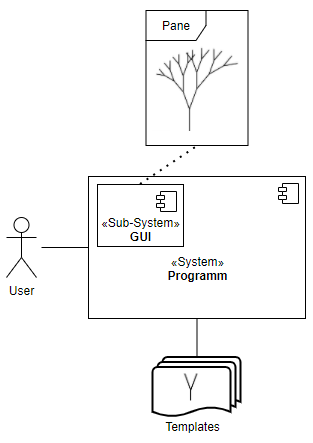
\includegraphics[width=6.2cm]{../images/Fachlicher_Kontext.PNG}
    \caption{System und Systemumgebung}
\end{figure}
\begin{figure}[H]
    \centering
    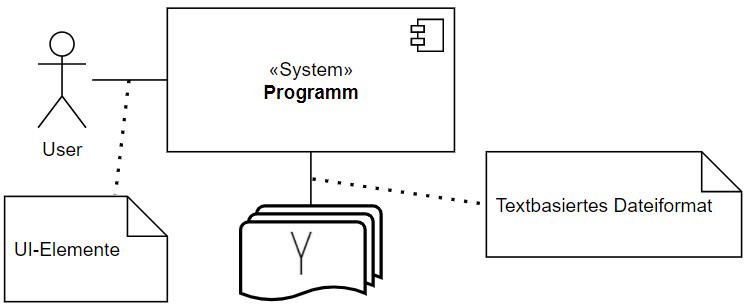
\includegraphics[width=10cm]{../images/Technischer_Kontext.PNG}
    \caption{Interaktion zwischen System und Systemumgebung}
\end{figure}

\subsection*{Bausteinsicht}
Der Benutzer interagiert über das User Interface mit dem Subsystem GUI, das sich mit der Visualisierung, dem Aufbau der
Eingabestruktur und dem Anlegen einer internen Baumtopologie beschäftigt.
Die Pipeline zum Erzeugen der Ausgabestrukturen beginnt mit dem Inferieren eines L-Systems aus der benutzerdefinierten
Struktur und gibt das erzeugte Ersetzungssystem an die folgende Komponente weiter.
Hierbei gilt der Pipeline-Kontext, welcher innerhalb der Pipeline an den jeweils nächsten Schritt weitergegeben und
dort aktualisiert wird, als Eingabe der Pipeline.
Hat die \texttt{Estimator}-Komponente eine Verteilung über Transformationsparameter angelegt, gilt der Kontext als
Ausgabe der Pipeline.

\underline{Ebene 1}
\begin{figure}[H]
    \centering
    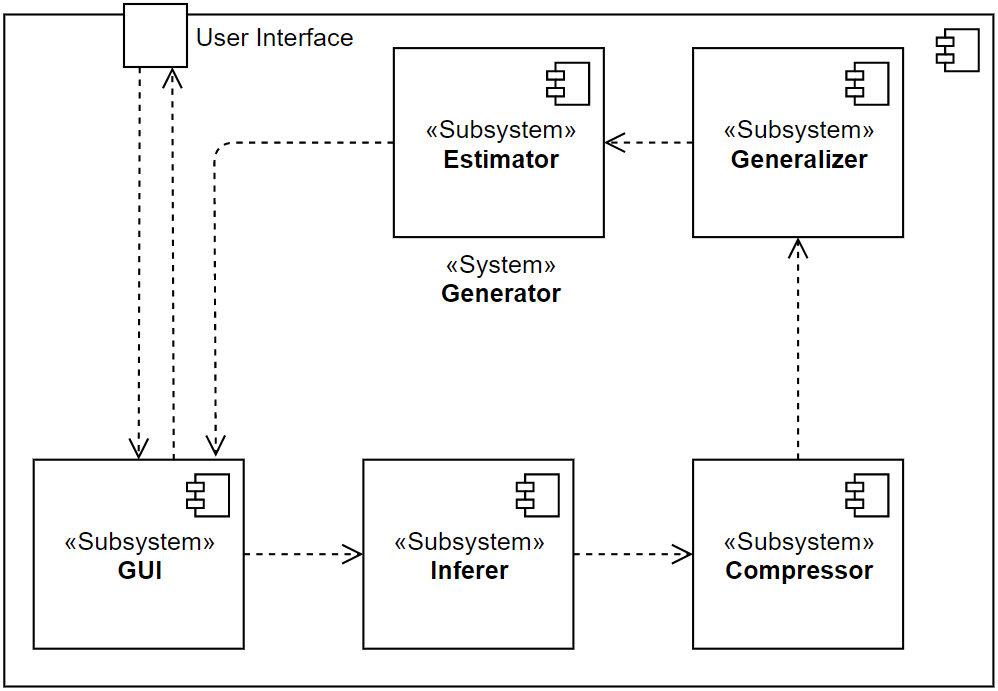
\includegraphics[width=12cm]{../images/Bausteinsicht_Ebene_1.PNG}
    \caption{Subsysteme mit fachlichen Abhängigkeiten}
\end{figure}

\newpage

Betrachtet man die GUI-Komponente genauer, setzt sich diese aus vier Subsystemen zusammen.
Das Application-Modul beschreibt den Einstiegspunkt des Programms.
Die grafische Benutzerschnittstelle wird aus einem View (Scene graph) mit zugehörigem Controller (Model)
aufgebaut.
Der Controller stellt die Logik für das View zur Verfügung.
Neben der Erstellung der Basisstruktur, wird die Baumstruktur in einer seperaten Komponente umgesetzt.

\underline{Ebene 2}
\begin{figure}[H]
    \centering
    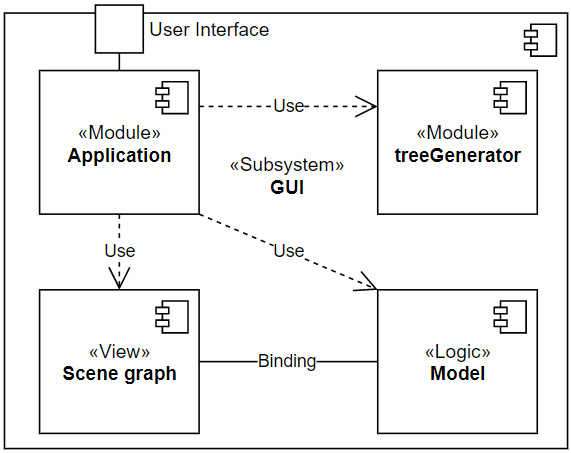
\includegraphics[width=9cm]{../images/Bausteinsicht_Ebene_2.PNG}
    \caption{Subsystem GUI}
\end{figure}

\newpage

\subsection*{Laufzeitsicht}
Aus der nachfolgenden Abbildung geht hervor, wie sich der Informationsfluss zwischen den einzelnen Subsystemen verhält.
Wird der Systemprozess einmal durchlaufen, besteht die Möglichkeit die Ausführung des generalisierten L-Systems mit
erneuter Vergabe der Transformationsparameter aus der Häufigkeitsverteilung der Estimator-Komponente zu starten.
Der Ablauf des Systems setzt sich wie folgt zusammen:

\begin{figure}[H]
    \centering
    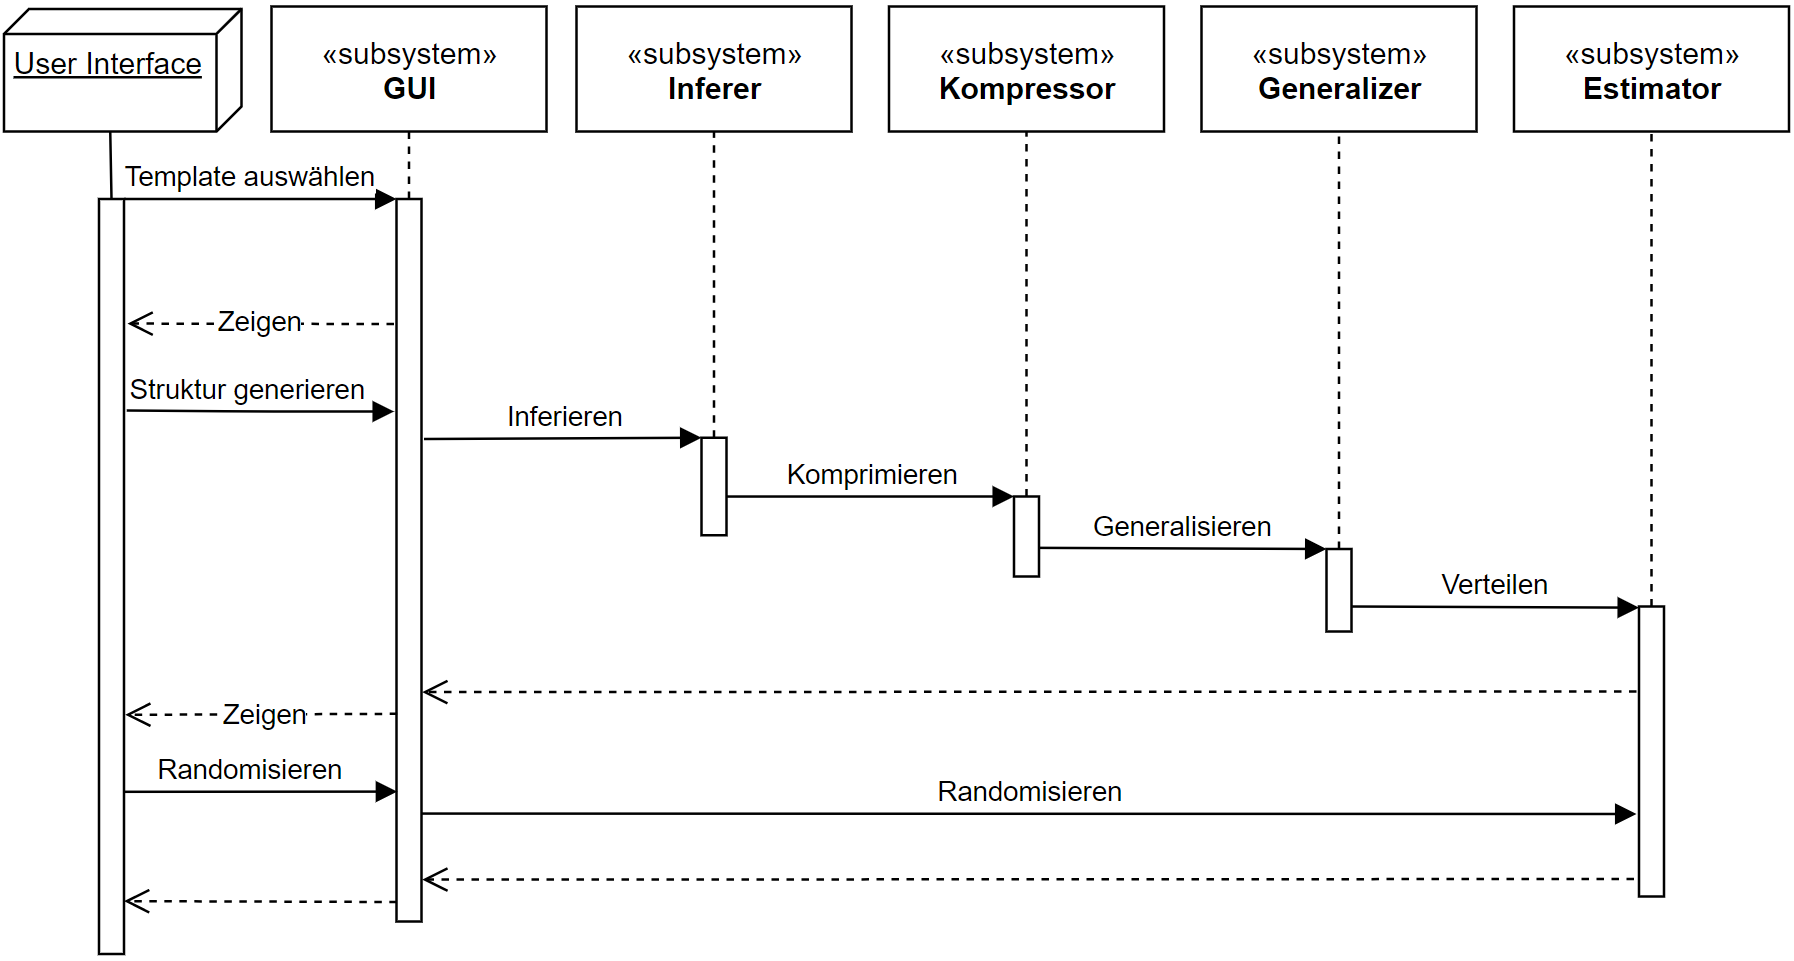
\includegraphics[width=14cm]{../images/Laufzeitsicht.PNG}
    \caption{Laufzeitsicht}
\end{figure}

\newpage

\subsection*{Verteilungssicht}
Die Ausführung des Programms wird durch ein einfaches Startskript zur Verfügung gestellt.
Die folgende Abbildung der Verteilungssicht stellt lediglich die Ausführung auf einer Windows-Maschine dar.

\begin{figure}[H]
    \centering
    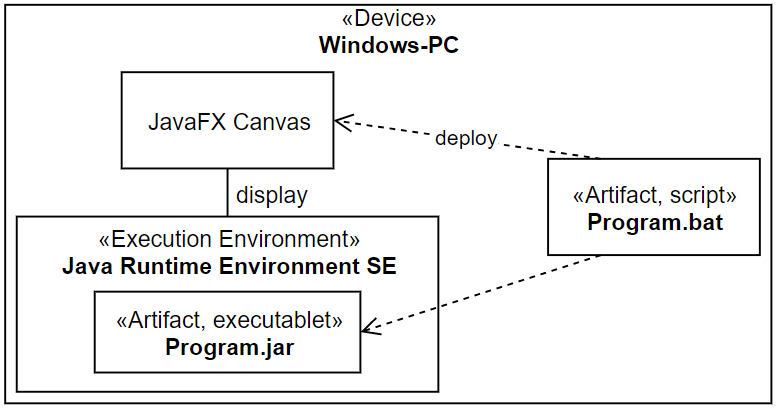
\includegraphics[width=10cm]{../images/Verteilungssicht.PNG}
    \caption{Infrastruktur Windows-PC}
\end{figure}

\subsection*{Datenstrukturen}
Das wesentliche Datenmodell ist als UML-Diagramm modelliert (siehe Seite~\pageref{anhang} Anhang).\\
Die während der Strukturierung entstehende Baumstuktur wird in~\ref{baum} gezeigt.\\
\texttt{TreeNode} implementiert das \texttt{Iterable}-Interface, sodass durch die Überladung der \texttt{iterate}-Funktion
ein Iterator zurückgegeben werden kann, der ein Durchgehen der Baumtopologie möglich macht.
Dieser Iterator ist durch die Klasse \mbox{\texttt{TreeNodeIterator}}, die das \texttt{Iterator}-Interface implementiert, definiert.
Die überladene \texttt{next}-Funktion beschreibt eine Iterierung des Baums durch eine Breitensuche.\\~\\
~\ref{pipeline} beschreibt den Generierungsprozess im Pipeline-Design-Pattern.
Jeder Teilschritt des Prozesses ist durch eine Klasse, die das \texttt{Pipe}-Interface nutzt, definiert.
Die überladene \texttt{process}-Funktion nimmt den \texttt{PipelineContext} entgegen, verändert diesen und gibt ihn
anschließend zurück.
Das \texttt{PipelineContext}-Objekt hält die Daten, die die eizelnen Schritte benötigen und zurückgeben (Pipeline-Kontext).\\
Die Pipes lassen sich in einer festen Reihenfolge durch die überladene \texttt{pipe}-Funktion\\eines
\texttt{Pipeline}-Objekts einreihen.
Die Prozesspipeline wird durch die \texttt{execute}-Funktion ausgeführt.\\~\\
Die verschiedenen Algorithmen zur Manipulation von L-Systemen werden in~\ref{tool} durch verschiedene Objekte definiert.
Sie werden in der entsprechenden Pipe erstellt und durch eine Funktion ausgeführt, die das veränderte L-System
zurückgibt.
Im Konstruktor werden benötige Daten aus dem Pipeline-Kontext an den Algorithmus übergeben.